\documentclass{article}
\usepackage{flowchart}
\usepackage{tikz}
\usetikzlibrary{shapes,arrows,chains}
\begin{document}
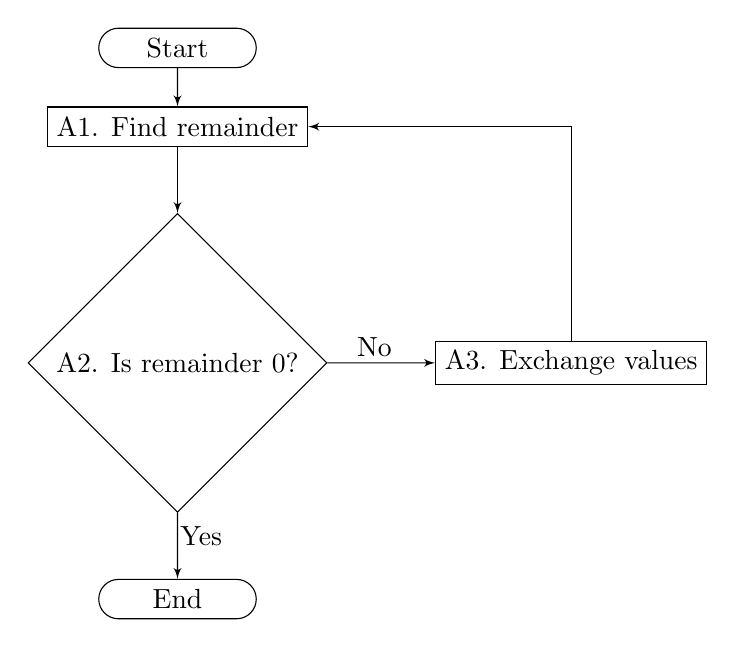
\begin{tikzpicture}[>=latex']
  \def\smbwd{2cm}
  \node (terminal1) at (0, 0) [draw, terminal, minimum width=\smbwd,
    minimum height=0.5cm] {Start};
  \node (process1) at (0, -1) [draw, process, minimum width=\smbwd,
    minimum height=0.5cm] {A1. Find remainder};
  \node (decision1) at (0, -4) [draw, decision, minimum width=1cm,
    minimum height=0.5cm] {A2. Is remainder 0?};
  \node (process2) at (5, -4) [draw, process, minimum width=\smbwd,
    minimum height=0.5cm] {A3. Exchange values};
  \node (terminal2) at (0, -7) [draw, terminal, minimum width=\smbwd,
    minimum height=0.5cm] {End};
  \draw[->] (terminal1) -- (process1);
  \draw[->] (process1) -- (decision1);
  \draw[->] (decision1) -- (process2);
  \draw[->] (decision1) -- (terminal2);
  \draw[->] (process2) |- (process1);
  \draw (2.5, -3.8) node{No};
  \draw (.3, -6.2) node{Yes};
\end{tikzpicture}
\end{document}
